\chapter{Algorithms}

Neural networks are a set of algorithms that identify patterns and are roughly modeled after the human brain. They use machine perception to categorize or organize raw information in order to better interpret sensory data. All real-world data, including pictures, sounds, texts, and time series, must be transformed into vectors in order to understand the numerical patterns inherent therein.

\section{Design Procedure} %  use this section 
\label{sec:intro_sum_results} % label of summary of results
                  
        Step 1: First, generate the dataset using the custom function from the y-finance package. &    \\        
        Step 2: Begin the solution feature extraction for 9 tickers with 1 ticker as the feature model.  &    \\        
        Step 3:Indicate the total selected and merged samples based on the multi-objective function with regard to the single ticker chosen.   &    \\
        Step 4: Normalize the entire data to improve accuracy and intuitive learning responses.  &    \\
        Step 5:Determine the overall featured labels, then design a TNN and ARIMA-ANN model for training.      &    \\
        Chapter 6 & Conclusions and Future Work  &    \\        
        Step 7: Visualize the data using 5 minute, 1 hour, and 1 day increments. &    \\      
        Step 8:Show the total error change on the single ticker using the appropriate highlighted data as (open (1 ticker)-open (9 tickers)).  & \\
Step 9:How the proposed and current algorithms affect the display of stock data dependent on the year. & \\

\section{Transformer Neural Networks}
In many neural network topologies, the transformer is used to handle sequential data such as natural language text, genetic sequences, auditory signals, or time series data. Transformer neural networks are most commonly employed for natural language processing. A transformer neural network can convert an input phrase as a series of vectors into an encoding vector, which it can then decode back into a sequence of vectors. The attention mechanism is an important component of the transformer. The attention mechanism determines the significance of other tokens in an input for encoding a certain token. The attention mechanism in a machine translation model, for example, allows the transformer to convert words such as "it" into a word of the proper gender in French or Spanish by paying attention to all relevant phrases in the original text. Importantly, the transformer may use the attention mechanism to determine how to translate a word by concentrating on phrases to the left and right of the current sentence. Transformer neural networks have replaced the previously used recurrent neural network (RNN), long short-term memory (LSTM), and gated recurrent (GRU) neural network designs.

Importantly, the transformer may use the attention mechanism to select how to translate a word by focusing on certain phrases to the left and right of the current sentence. Transformer neural networks have taken the role of previous neural network architectures such as recurrent neural network (RNN), long short-term memory (LSTM), and gated recurrent (GRU).

\section {Transformer Neural Network Design}

\begin{figure}[ht]
    \centering
    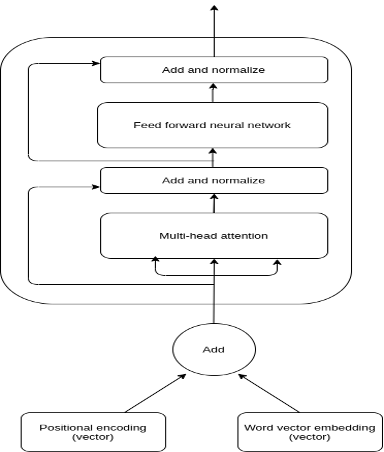
\includegraphics[scale=0.7]{figures/Transformer.png}
    \caption{The architecture of a transformer neural network.}
    \label{fig:chart_a}
\end{figure}

The transformer neural network takes a phrase as input and divides it into two sequences: one with word vector embeddings and one with positional encodings. The text is represented mathematically using word vector embeddings. Words must first be translated to embedding format before they can be processed by a neural network. In the embedding representation, each dictionary word is represented by a vector. Positional encodings are vector representations of the word's original location inside the sentence.The transformer combines word vector embeddings and positional encodings before passing the resulting data through a variety of encoders and decoders. It should be emphasized that, unlike RNNs and LSTMs, the entire input is sent into the network at once, rather than one piece at time.

Each encoder converts the input into a new collection of vectors known as an encoding. The decoders do the inverse, turning the encodings into a set of probabilities for possible output words. The SoftMax function may be used to represent the output probabilities in another natural language phrase. The attention mechanism, which is included in all encoders and decoders, allows the processing of one input word to integrate relevant data from other words while masking the words that do not contain significant information. This must be calculated several times, thus we use the parallel computing capabilities given by GPUs to build various attention strategies. The multi-head attention mechanism is to blame. Transformers have an advantage over LSTMs and RNNs in that they can analyze many words at the same time.




\section{Autoregressive Integrated Moving Average (ARIMA)}

It is a statistical analysis model that uses time series data to either better comprehend the data or forecast future trends. A statistical model is autoregressive if it predicts future values based on previous values. For example, an ARIMA model may attempt to estimate a stock's future pricing based on its past performance or a company's earnings based on previous periods.

ARIMA's components serve as parameters using standard notation. A conventional nomenclature for ARIMA models is ARIMA with p, d, and q, where integer values represent the parameters to denote the kind of ARIMA model utilized. Parameters can be specified as: 1
\begin{figure}[ht]
    \centering
    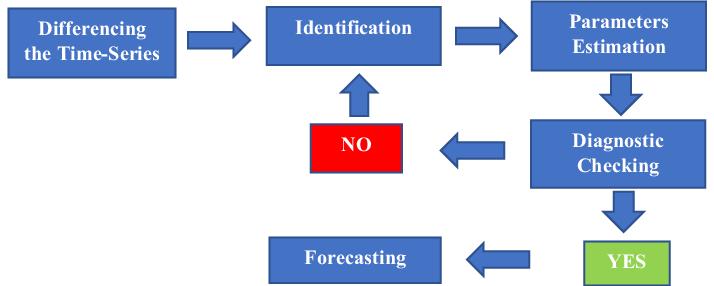
\includegraphics[scale=0.5]{figures/Arima.png}
    \caption{The architecture of a ARIMA neural network.}
    \label{fig:chart_a}
\end{figure}

p is the number of lag observations in the model, commonly known as the lag order.
d: the number of times the raw observations are differentiated; also known as the degree of differencing.
q is the size of the moving average window, commonly known as the moving average's order.
To start creating an ARIMA model for an investment, you download as much price data as possible. After identifying the data patterns, you look at the autocorrelations to determine the lowest order of differencing (d). If the lag-1 autocorrelation is zero or negative, the series is already differentiated. If the lag-1 is more than zero, you may need to differentiate the series further.

Next, compare autocorrelations and partial autocorrelations to establish the order of regression (p) and the order of the moving average. Once you have the necessary information, you may pick the model you will use.

\section{Artificial Neural Networks (ANN)}
Artificial Neural Networks (ANN) are algorithms that simulate brain activity and are used to model complex patterns and foresee problems. The Artificial Neural Network (ANN) is a deep learning technique based on the notion of biological neural networks in the human brain. An attempt to imitate the workings of the human brain led to the development of artificial neural networks (ANN). ANNs operate very similarly to biological neural networks, however they are not identical. The ANN algorithm only takes numbers and structured input.

\begin{figure}[ht]
    \centering
    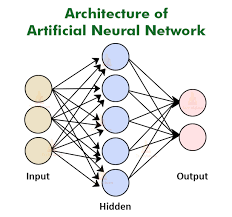
\includegraphics[scale=1]{figures/ANN.png}
    \caption{The architecture of a ANN neural network.}
    \label{fig:chart_a}
\end{figure}

Image, Text, and Speech are examples of unstructured and non-numeric data types that are accepted by Convolutional Neural Networks (CNN) and Recursive Neural Networks (RNN). This page only discusses Artificial Neural Networks. The majority of neural networks have units that connect one layer to the next. Each of these links has a weight, which determines how one unit affects another. As input is sent from one unit to another, the neural network learns more about the data, finally producing an output from the output layer. 









